\documentclass[aspectratio=169, 12pt]{beamer}

% === THEME ET COULEURS ===
\usetheme{Madrid}
\usecolortheme{default}

\definecolor{upblue}{RGB}{0, 75, 135}
\definecolor{darkblue}{RGB}{0, 50, 100}
\definecolor{lightgray}{RGB}{245, 245, 245}

\setbeamercolor{structure}{fg=upblue}
\setbeamercolor{palette primary}{bg=upblue, fg=white}
\setbeamercolor{palette secondary}{bg=darkblue, fg=white}
\setbeamercolor{palette tertiary}{bg=upblue, fg=white}
\setbeamercolor{frametitle}{bg=upblue!8, fg=upblue}
\setbeamercolor{title}{fg=white, bg=upblue}
\setbeamercolor{block title}{bg=upblue, fg=white}
\setbeamercolor{block body}{bg=upblue!5}
\setbeamercolor{block title alerted}{bg=red!70!black, fg=white}
\setbeamercolor{block body alerted}{bg=red!5}
\setbeamercolor{item}{fg=upblue}

\setbeamertemplate{navigation symbols}{}
\setbeamertemplate{footline}{%
  \hfill\insertframenumber/\inserttotalframenumber\hspace{0.5cm}\vspace{0.3cm}
}

% === PACKAGES ===
\usepackage[utf8]{inputenc}
\usepackage[T1]{fontenc}
\usepackage[french]{babel}
\usepackage{graphicx}
\graphicspath{{figures/}}
\usepackage{booktabs}
\usepackage{multirow}
\usepackage{array}
\usepackage{colortbl}
\usepackage{amsmath}
\usepackage{tikz}
\usetikzlibrary{arrows.meta, shapes.geometric, positioning, calc, fit, backgrounds}
\usepackage{hyperref}

% === MACROS ===
\newcommand{\positif}[1]{\textcolor{green!60!black}{#1}}
\newcommand{\negatif}[1]{\textcolor{red!70!black}{#1}}
\newcommand{\neutre}[1]{\textcolor{gray}{#1}}

% === INFORMATIONS ===
\title[GeoR2LLMs]{GeoR2LLMs}
\subtitle{Syst\`eme Question-R\'eponse en G\'eographie\\avec G\'en\'eration Augment\'ee par la Recherche d'Information}
\author{Mohamed DIALLO \and Hiba L'MOUDDEN \and Feras MAKHLOUF \and Osama BAAZZI \and Ousama BOUTEZROUT}
\institute{Master 2 Intelligence Artificielle\\Universit\'e Paul Sabatier -- Toulouse III}
\date{Mars 2026}
\titlegraphic{\vspace{-0.5cm}
\includegraphics[width=2.5cm]{logo_univ_toulouse}}

\begin{document}

% ============================================================
% PAGE DE TITRE
% ============================================================
\begin{frame}[plain]
  \titlepage
\end{frame}

% ============================================================
% PLAN
% ============================================================
\begin{frame}{Plan}
  \tableofcontents
\end{frame}

% ============================================================
% 1. INTRODUCTION
% ============================================================
\section{Introduction}

\begin{frame}{Contexte et motivation}
  \begin{block}{Probl\'ematique}
    Les LLMs peinent \`a restituer des connaissances g\'eographiques pr\'ecises
    et \`a raisonner spatialement, m\^eme avec une temp\'erature de z\'ero.
  \end{block}

  \vspace{0.2cm}

  \begin{itemize}
    \item Mod\`eles $\leq$ 3B particuli\`erement limit\'es en connaissances factuelles
    \item Le \textbf{RAG} promet de compenser ces lacunes via un contexte externe
    \item \textbf{Question\,:} Le RAG am\'eliore-t-il r\'eellement le QA g\'eographique\,?
  \end{itemize}

  \vspace{0.2cm}

  \begin{alertblock}{Objectif}
    Impl\'ementer et \'evaluer un syst\`eme QA g\'eographique en configuration RAG, en comparant syst\'ematiquement Baseline et RAG.
  \end{alertblock}
\end{frame}

\begin{frame}{Organisation du travail}
  \begin{columns}[T]
    \begin{column}{0.48\textwidth}
      \begin{block}{\'Etape 1 -- Plateforme de base}
        \begin{itemize}
          \item 1 LLM (Qwen3-0.6B)
          \item 1 dataset (GeoSQA)
          \item 1 corpus (Wikipedia FR)
          \item Objectif\,: pipeline fonctionnel + baseline
        \end{itemize}
      \end{block}
    \end{column}
    \begin{column}{0.48\textwidth}
      \begin{block}{\'Etape 2 -- Exploration}
        \begin{itemize}
          \item 4 LLMs exploitables (+1 incompatible)
          \item 3 datasets g\'eographiques
          \item Analyse factorielle crois\'ee
          \item Objectif\,: identifier les facteurs de performance
        \end{itemize}
      \end{block}
    \end{column}
  \end{columns}

  \vspace{0.4cm}
  \centering
  \small
  \textit{Environnement\,: Google Colab, GPU NVIDIA T4 (16\,Go VRAM)}
\end{frame}

% ============================================================
% 2. RAPPEL THEORIQUE
% ============================================================
\section{Rappel th\'eorique}

\begin{frame}{Fondements th\'eoriques}
  \begin{columns}[T]
    \begin{column}{0.48\textwidth}
      \begin{block}{LLMs -- Transformer}
        \small
        \begin{itemize}
          \item Attention multi-t\^etes\,:\\
            $\text{Att}(Q,K,V) = \text{softmax}\!\left(\frac{QK^\top}{\sqrt{d_k}}\right)\!V$
          \item G\'en\'eration autor\'egressive (d\'ecodeur)
          \item Capacit\'es \'emergentes (CoT, in-context learning)
        \end{itemize}
      \end{block}
    \end{column}
    \begin{column}{0.48\textwidth}
      \begin{block}{RAG na\"if (Retrieve-then-Read)}
        \small
        \begin{itemize}
          \item LLMs ne stockent pas toutes les connaissances factuelles
          \item RAG externalise la m\'emoire dans un corpus
          \item Injection directe des documents dans le prompt
        \end{itemize}
      \end{block}
    \end{column}
  \end{columns}

  \vspace{0.1cm}
  \small
  \textbf{QA g\'eographique\,:} raisonnement spatial + connaissances encyclop\'ediques.
  Aucun LLM actuel ne raisonne de mani\`ere fiable sur les directions cardinales $\Rightarrow$ int\'er\^et du RAG.
\end{frame}

% ============================================================
% 3. ARCHITECTURE
% ============================================================
\section{Architecture du syst\`eme}

\begin{frame}{Pipeline RAG -- Vue d'ensemble}
  \begin{center}
    \resizebox{0.95\textwidth}{!}{%
    \begin{tikzpicture}[
      node distance=1cm and 1.5cm,
      box/.style={rectangle, draw, rounded corners=4pt, minimum height=1cm, minimum width=2.5cm, align=center, font=\small},
      data/.style={box, fill=blue!8, draw=blue!40},
      process/.style={box, fill=green!8, draw=green!40},
      model/.style={box, fill=orange!10, draw=orange!40},
      result/.style={box, fill=red!8, draw=red!40},
      arrow/.style={-{Stealth[length=2.5mm]}, thick, draw=gray!70},
      lbl/.style={font=\scriptsize\itshape, text=gray}
    ]
      \node[data] (corpus) {Corpus\\{\scriptsize Wikipedia / Reviews}};
      \node[data, below=1.2cm of corpus] (question) {Question\\{\scriptsize GeoSQA / GKMC / Tourism-QA}};
      \node[process, right=1.5cm of corpus] (chunk) {Chunking\\{\scriptsize 512 car., overlap 50}};
      \node[model, right=1.2cm of chunk] (bge) {BGE-m3\\{\scriptsize 1024 dim.}};
      \node[process, right=1.2cm of bge] (faiss) {FAISS\\{\scriptsize IndexFlatIP}};
      \node[model, right=1.5cm of question] (encq) {Encodage\\{\scriptsize question}};
      \node[process, right=3.5cm of encq] (topk) {Top-K\\{\scriptsize K=5}};
      \node[model, below=1.2cm of topk, xshift=-2cm] (llm) {LLM\\{\scriptsize Generator}};
      \node[result, right=1.2cm of llm] (rep) {R\'eponse};

      \draw[arrow] (corpus) -- (chunk);
      \draw[arrow] (chunk) -- (bge);
      \draw[arrow] (bge) -- node[above, lbl] {embeddings} (faiss);
      \draw[arrow] (question) -- (encq);
      \draw[arrow] (encq) -- node[above, lbl] {vecteur} (topk);
      \draw[arrow] (faiss) -- node[right, lbl] {index} (topk);
      \draw[arrow] (topk) -- node[right, lbl] {contexte} (llm);
      \draw[arrow] (question.south) |- (llm.west);
      \draw[arrow] (llm) -- (rep);

      \begin{scope}[on background layer]
        \node[fit=(chunk)(bge)(faiss), draw=green!60, dashed, rounded corners=6pt, inner sep=8pt, label={[font=\small\bfseries, text=green!50!black]above:Retriever}] {};
        \node[fit=(llm)(rep), draw=orange!60, dashed, rounded corners=6pt, inner sep=8pt, label={[font=\small\bfseries, text=orange!50!black]below:Generator}] {};
      \end{scope}
    \end{tikzpicture}
    }
  \end{center}
\end{frame}

\begin{frame}{Composants cl\'es}
  \begin{columns}[T]
    \begin{column}{0.48\textwidth}
      \begin{block}{Retriever}
        \begin{itemize}
          \item \textbf{BGE-m3} (BAAI) -- embeddings multilingues, 1024 dimensions
          \item \textbf{FAISS} IndexFlatIP -- similarit\'e cosinus
          \item Chunks de 512 car., overlap 50
          \item Top-K = 5 documents
        \end{itemize}
      \end{block}
    \end{column}
    \begin{column}{0.48\textwidth}
      \begin{block}{Generator}
        \begin{itemize}
          \item Prompt syst\`eme\,: expert g\'eographie
          \item Mode Baseline\,: pas de contexte
          \item Mode RAG\,: top-5 documents inject\'es
          \item Extraction regex de la lettre (A/B/C/D)
        \end{itemize}
      \end{block}
    \end{column}
  \end{columns}

  \vspace{0.2cm}

  \begin{block}{Evaluator}
    \small
    \textbf{G\'en\'eration\,:} Accuracy MCQ, Exact Match, F1 \quad
    \textbf{Retrieval\,:} Hit Rate@K, MRR@K \quad
    \textbf{Tourism-QA\,:} Accuracy@1, F1 POI
  \end{block}
\end{frame}

\begin{frame}{Prompt Baseline vs RAG}
  \begin{columns}[T]
    \begin{column}{0.47\textwidth}
      \begin{block}{Mode Baseline (sans contexte)}
        \small
        \texttt{system:} \textit{Tu es un expert en g\'eographie. R\'eponds uniquement avec la lettre correcte.}\\[0.2cm]
        \texttt{user:} \textit{Question: \{question\}\\Options: A) ... B) ... C) ... D) ...}
      \end{block}
    \end{column}
    \begin{column}{0.47\textwidth}
      \begin{block}{Mode RAG (avec contexte)}
        \small
        \texttt{system:} \textit{Tu es un expert en g\'eographie. R\'eponds uniquement avec la lettre correcte.}\\[0.2cm]
        \texttt{user:} \textit{\textbf{Contexte: \{top-5 documents\}}\\Question: \{question\}\\Options: A) ... B) ... C) ... D) ...}
      \end{block}
    \end{column}
  \end{columns}

  \vspace{0.3cm}

  \centering
  La seule diff\'erence\,: l'injection des \textbf{top-5 documents} r\'ecup\'er\'es par le retriever.\\
  Cela permet d'isoler pr\'ecis\'ement l'\textbf{effet du RAG} sur la performance.
\end{frame}

% ============================================================
% 4. METHODOLOGIE
% ============================================================
\section{M\'ethodologie}

\begin{frame}{Mod\`eles \'evalu\'es}
  \begin{table}
    \centering
    \small
    \begin{tabular}{@{} l l c c @{}}
      \toprule
      \textbf{Mod\`ele} & \textbf{Famille} & \textbf{Taille} & \textbf{Statut} \\
      \midrule
      Qwen3-0.6B & Qwen (Alibaba) & 0.6B & \positif{OK} \\
      Qwen3-1.7B & Qwen (Alibaba) & 1.7B & \positif{OK} \\
      Llama-3.2-1B-Instruct & Llama (Meta) & 1.0B & \positif{OK} \\
      Llama-3.2-3B-Instruct & Llama (Meta) & 3.0B & \positif{OK} \\
      Ministral-3-3B-Instruct & Mistral & 3.0B & \negatif{Incompatible} \\
      \bottomrule
    \end{tabular}
  \end{table}

  \vspace{0.2cm}

  \begin{alertblock}{Ministral-3-3B -- Incompatibilit\'e technique}
    \texttt{Mistral3Config} est une architecture vision-langage multimodale, incompatible avec \texttt{AutoModelForCausalLM} (mod\`eles textuels).
  \end{alertblock}
\end{frame}

\begin{frame}{Datasets g\'eographiques}
  \begin{table}
    \centering
    \small
    \begin{tabular}{@{} l c c l l @{}}
      \toprule
      \textbf{Dataset} & \textbf{$N$} & \textbf{Langue} & \textbf{T\^ache} & \textbf{Corpus RAG} \\
      \midrule
      GeoSQA & 200 & ZH $\to$ EN & QCM & Wikipedia FR \\
      GKMC & 200 & EN natif & QCM & Wikipedia FR \\
      Tourism-QA & 100 & EN & Reco. POI & Reviews EN \\
      \bottomrule
    \end{tabular}
  \end{table}

  \vspace{0.3cm}

  \begin{columns}[T]
    \begin{column}{0.32\textwidth}
      \centering
      \textbf{GeoSQA}\\
      \small Raisonnement spatial, lyc\'ee chinois, traduit EN
    \end{column}
    \begin{column}{0.32\textwidth}
      \centering
      \textbf{GKMC}\\
      \small Connaissances encyclop\'ediques, nativement EN
    \end{column}
    \begin{column}{0.32\textwidth}
      \centering
      \textbf{Tourism-QA}\\
      \small Recommandation de POI, reviews utilisateurs
    \end{column}
  \end{columns}
\end{frame}

% ============================================================
% ORGANISATION
% ============================================================
\section{Organisation et Gestion du Projet}

\begin{frame}{Stratégie Méthodologique et Approche Agile}
    \begin{itemize}
        \item \textbf{Agilité adaptée} : Découpage du travail en sprints de production de connaissances pour maintenir la continuité scientifique.
        \item \textbf{Synchronisation} : 
        \begin{itemize}
            \item Réunions hebdomadaires (Google Meet) pour les points de blocage.
            \item Échanges opérationnels quotidiens (WhatsApp).
        \end{itemize}
        \item \textbf{Reproductibilité} :
        \begin{itemize}
            \item Mise en place précoce de l'infrastructure sur GitHub.
            \item Versioning du code, des prompts et des configurations.
        \end{itemize}
        \item \textbf{Maîtrise des risques} : Identification rapide des limites du RAG naïf permettant un pivot vers une architecture hybride sans retard.
    \end{itemize}
\end{frame}

\begin{frame}{Organisation Fonctionnelle de l'Équipe}
    Afin de responsabiliser chaque membre sur un verrou scientifique, l'équipe s'est structurée par pôles d'expertise (selon une matrice RACI) :
    \vspace{0.4cm}
    \begin{itemize}
        \item \textbf{Pilotage Scientifique} : Lynda TAMINE-LECHANI
        \item \textbf{Coordination \& Intégration} : Feras MAKHLOUF
        \item \textbf{Génie Logiciel \& RAG} : Hiba L'MOUDDEN
        \item \textbf{Raisonnement Spatial} : Mohamed DIALLO \& Ousama BOUTEZROUT
        \item \textbf{Audit \& Évaluation} : Osama BAAZZI
    \end{itemize}
\end{frame}

\begin{frame}{Planification Temporelle (Gantt)}
    \textbf{Stratégie} : Parallélisation entre une phase de recherche théorique étendue et une accélération expérimentale en fin de projet.
    \vspace{0.3cm}
    \begin{table}[]
        \centering
        \small
        \renewcommand{\arraystretch}{1.5}
        \begin{tabular}{|c|p{8.5cm}|}
            \hline
            \textbf{Période} & \textbf{Objectifs de la phase} \\ \hline
            \textbf{Bloc 1 \& 2} (S1-S4) & \textbf{Gestion des flux} : Acquisition théorique, état de l'art et curation du corpus. \\ \hline
            \textbf{Bloc 3} (S5-S6) & \textbf{Pivot Expérimental} : Évaluations, optimisation du RAG, intégration Tool-Use et architecture hybride. \\ \hline
            \textbf{Bloc 4} (S7-S8) & \textbf{Audit de Qualité} : Benchmark "End-to-End", réduction de la dette technique et peer-review finale. \\ \hline
        \end{tabular}
    \end{table}
\end{frame}
% ============================================================
% 4. RESULTATS ETAPE 1
% ============================================================
\section{R\'esultats -- \'Etape 1}

\begin{frame}{\'Etape 1 -- Stabilit\'e du prompt (Qwen3-0.6B, 50 questions)}
  \begin{table}
    \centering
    \begin{tabular}{@{} c l c @{}}
      \toprule
      \textbf{Rang} & \textbf{Strat\'egie} & \textbf{Accuracy} \\
      \midrule
      1 & P1 -- Prompt basique (FR) & \textbf{52.0\,\%} \\
      2 & P4 -- Few-Shot 2 exemples & 38.0\,\% \\
      2 & P5 -- Prompt basique (EN) & 38.0\,\% \\
      4 & P2 -- Expert contraint (FR) & 30.0\,\% \\
      5 & P3 -- Chain-of-Thought & 20.0\,\% \\
      \midrule
      & \textit{Seuil al\'eatoire} & 25.0\,\% \\
      \bottomrule
    \end{tabular}
  \end{table}

  \vspace{0.2cm}

  \begin{itemize}
    \item \'Ecart de \textbf{32 points} entre P1 et P3 -- forte sensibilit\'e au prompt
    \item Le CoT d\'egrade sous le seuil al\'eatoire (20\,\%) -- inefficace pour 0.6B
    \item \textbf{Prompt P2} retenu malgr\'e un score inf\'erieur\,: il impose la lettre seule en sortie, garantissant une extraction fiable par regex
  \end{itemize}
\end{frame}

\begin{frame}{\'Etape 1 -- Baseline vs RAG (200 questions GeoSQA)}
  \begin{columns}[T]
    \begin{column}{0.45\textwidth}
      \begin{table}
        \centering
        \small
        \begin{tabular}{@{} l c c @{}}
          \toprule
          \textbf{M\'etrique} & \textbf{Base.} & \textbf{RAG} \\
          \midrule
          Accuracy & 0.245 & \positif{0.270} \\
          F1 Score & 0.030 & \negatif{0.011} \\
          Temps (s) & 353.6 & 495.6 \\
          \midrule
          HR@5 & -- & 0.080 \\
          MRR@5 & -- & 0.053 \\
          \bottomrule
        \end{tabular}
      \end{table}
    \end{column}
    \begin{column}{0.52\textwidth}
      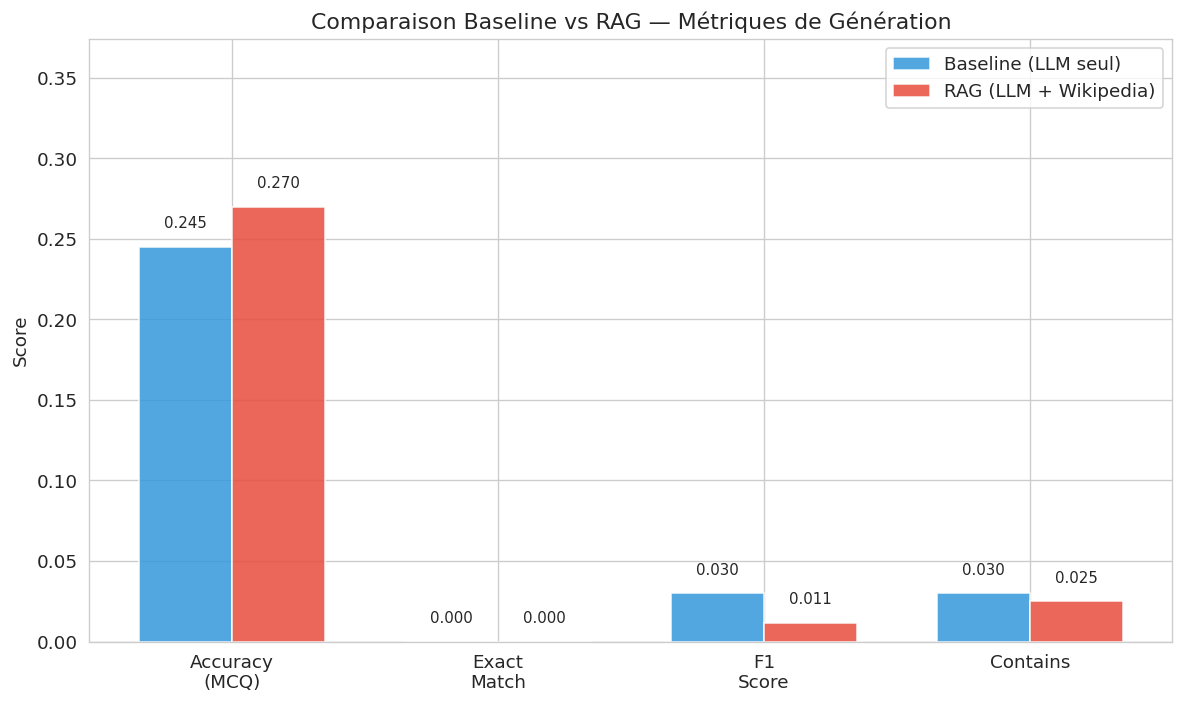
\includegraphics[width=\textwidth]{fig1_baseline_vs_rag.png}
    \end{column}
  \end{columns}

  \vspace{0.3cm}

  \begin{itemize}
    \item Accuracy\,: \positif{+10.2\,\%} relatif (5 questions de plus sur 200)
    \item Mais F1 chute de \negatif{-61.7\,\%} (corpus FR $\to$ r\'eponses en fran\c{c}ais)
    \item HR@5 = 8\,\% $\Rightarrow$ \textbf{92\,\%} des requ\^etes sans document pertinent
  \end{itemize}
\end{frame}

\begin{frame}{\'Etape 1 -- Biais de position et analyse qualitative}
  \begin{columns}[T]
    \begin{column}{0.48\textwidth}
      \begin{block}{Biais de position (Baseline)}
        \centering
        \begin{tabular}{@{} l c c @{}}
          \toprule
          \textbf{Lettre} & \textbf{$N$ pr\'edictions} & \textbf{\%} \\
          \midrule
          A & 123 & \negatif{61.5\,\%} \\
          B & 8 & 4.0\,\% \\
          C & 10 & 5.0\,\% \\
          D & 59 & 29.5\,\% \\
          \midrule
          \textit{Attendu} & 50 & 25.0\,\% \\
          \bottomrule
        \end{tabular}

        \vspace{0.2cm}
        \small Le mod\`ele 0.6B se rabat sur la premi\`ere option par d\'efaut.
      \end{block}
    \end{column}
    \begin{column}{0.48\textwidth}
      \begin{block}{R\'epartition qualitative (200 q.)}
        \centering
        \begin{tabular}{@{} l c @{}}
          \toprule
          \textbf{Cat\'egorie} & \textbf{\%} \\
          \midrule
          \rowcolor{gray!10}
          Double \'echec & 68.5\,\% \\
          Les deux corrects & 20.0\,\% \\
          \rowcolor{green!8}
          RAG sauve & 7.0\,\% \\
          \rowcolor{red!8}
          RAG trompe & 4.5\,\% \\
          \bottomrule
        \end{tabular}

        \vspace{0.2cm}
        \small Le double \'echec domine\,: l'info est absente du corpus.
      \end{block}
    \end{column}
  \end{columns}
\end{frame}

\begin{frame}{\'Etape 1 -- Facteurs limitants identifi\'es}
  \begin{table}
    \centering
    \small
    \begin{tabular}{@{} l c p{7cm} @{}}
      \toprule
      \textbf{Facteur} & \textbf{Impact} & \textbf{Observation} \\
      \midrule
      \rowcolor{red!10}
      Mismatch linguistique & Critique & Questions EN, corpus FR. HR@5 = 8\,\% \\
      \rowcolor{orange!10}
      Couverture th\'ematique & Important & G\'eo chinoise absente de Wikipedia FR \\
      \rowcolor{orange!10}
      Taille du LLM & Important & 0.6B $\approx$ seuil al\'eatoire (24.5\,\%) \\
      \rowcolor{orange!10}
      Biais de position & Important & Lettre A pr\'edite dans 61.5\,\% des cas \\
      \bottomrule
    \end{tabular}
  \end{table}

  \vspace{0.4cm}

  \begin{center}
    $\Longrightarrow$ Ces facteurs motivent l'\textbf{\'etape 2}\,: mod\`eles plus grands, datasets vari\'es, corpus align\'es.
  \end{center}
\end{frame}

% ============================================================
% 5. RESULTATS ETAPE 2
% ============================================================
\section{R\'esultats -- \'Etape 2}

\begin{frame}{GeoSQA -- Raisonnement spatial (200 questions)}
  \begin{columns}[T]
    \begin{column}{0.50\textwidth}
      \begin{table}
        \centering
        \scriptsize
        \begin{tabular}{@{} l c c c @{}}
          \toprule
          \textbf{Mod\`ele} & \textbf{Base.} & \textbf{RAG} & \textbf{$\Delta_{rel}$} \\
          \midrule
          Qwen3-1.7B & 0.390 & \textbf{0.335} & \negatif{-14.1\,\%} \\
          Qwen3-0.6B & 0.275 & 0.260 & \negatif{-5.5\,\%} \\
          Llama-3.2-3B & 0.270 & 0.230 & \negatif{-14.8\,\%} \\
          Llama-3.2-1B & 0.275 & 0.205 & \negatif{-25.5\,\%} \\
          \bottomrule
        \end{tabular}
      \end{table}
    \end{column}
    \begin{column}{0.48\textwidth}
      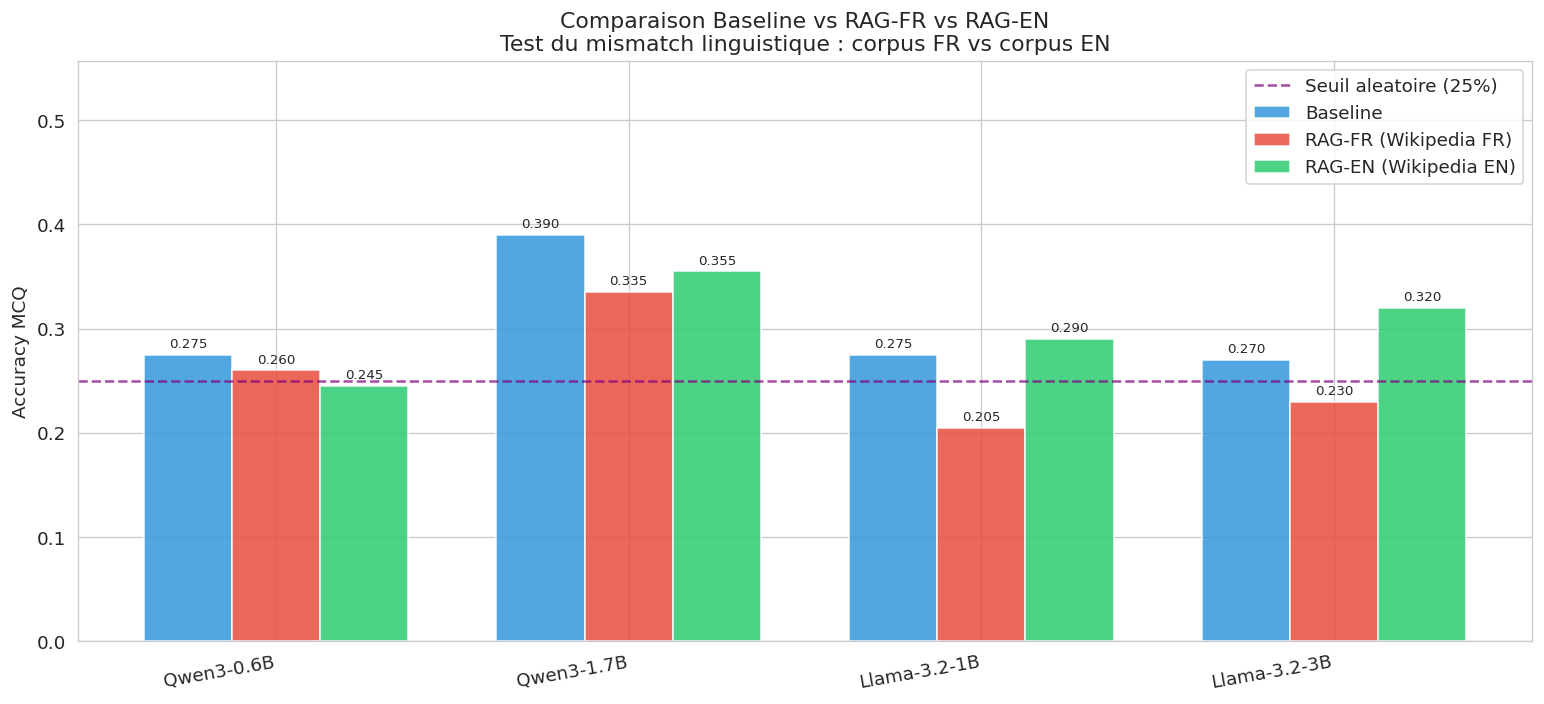
\includegraphics[width=\textwidth]{fig1_baseline_ragfr_ragen.png}
    \end{column}
  \end{columns}

  \vspace{0.3cm}

  \begin{alertblock}{Constat}
    Le RAG d\'egrade \textbf{tous les mod\`eles sans exception} sur GeoSQA.\\
    HR@5 = 0.060 -- le retriever ne trouve quasi rien (mismatch FR/EN).
  \end{alertblock}
\end{frame}

\begin{frame}{GKMC -- Connaissances encyclop\'ediques (200 questions)}
  \begin{columns}[T]
    \begin{column}{0.50\textwidth}
      \begin{table}
        \centering
        \scriptsize
        \begin{tabular}{@{} l c c c @{}}
          \toprule
          \textbf{Mod\`ele} & \textbf{Base.} & \textbf{RAG} & \textbf{$\Delta_{rel}$} \\
          \midrule
          Qwen3-1.7B & 0.585 & \textbf{0.605} & \positif{+3.4\,\%} \\
          Llama-3.2-3B & 0.565 & 0.485 & \negatif{-14.2\,\%} \\
          Qwen3-0.6B & 0.420 & 0.415 & \negatif{-1.2\,\%} \\
          Llama-3.2-1B & 0.330 & 0.335 & \positif{+1.5\,\%} \\
          \bottomrule
        \end{tabular}
      \end{table}
    \end{column}
    \begin{column}{0.48\textwidth}
      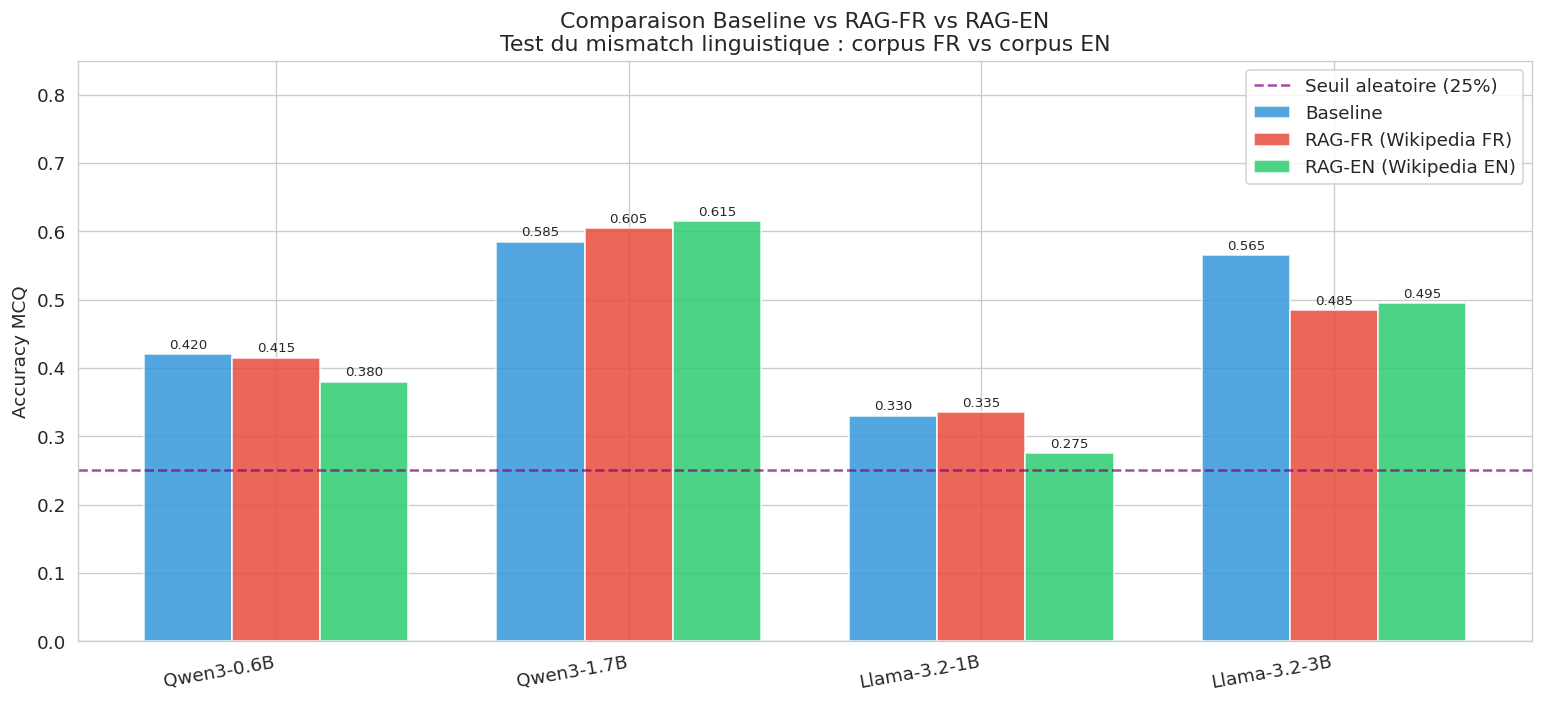
\includegraphics[width=\textwidth]{phase2b_fig1_baseline_ragfr_ragen.png}
    \end{column}
  \end{columns}

  \vspace{0.15cm}

  \begin{block}{Observations}
    \begin{itemize}
      \item Qwen3-1.7B atteint \textbf{0.605} -- meilleur score absolu du projet
      \item Llama-3.2-3B\,: forte d\'egradation malgr\'e de bonnes connaissances internes
      \item Le contexte non pertinent d\'estabilise les mod\`eles performants
    \end{itemize}
  \end{block}
\end{frame}

\begin{frame}{Tourism-QA -- Recommandation de POI (100 questions)}
  \begin{columns}[T]
    \begin{column}{0.50\textwidth}
      \begin{table}
        \centering
        \scriptsize
        \begin{tabular}{@{} l c c c @{}}
          \toprule
          \textbf{Mod\`ele} & \textbf{Base.} & \textbf{RAG} & \textbf{$\Delta_{rel}$} \\
          \midrule
          Qwen3-1.7B & 0.590 & 0.590 & 0.0\,\% \\
          Qwen3-0.6B & 0.560 & 0.570 & \positif{+1.8\,\%} \\
          Llama-3.2-3B & \textbf{0.700} & 0.540 & \negatif{-22.9\,\%} \\
          Llama-3.2-1B & 0.520 & 0.410 & \negatif{-21.2\,\%} \\
          \bottomrule
        \end{tabular}
      \end{table}
    \end{column}
    \begin{column}{0.48\textwidth}
      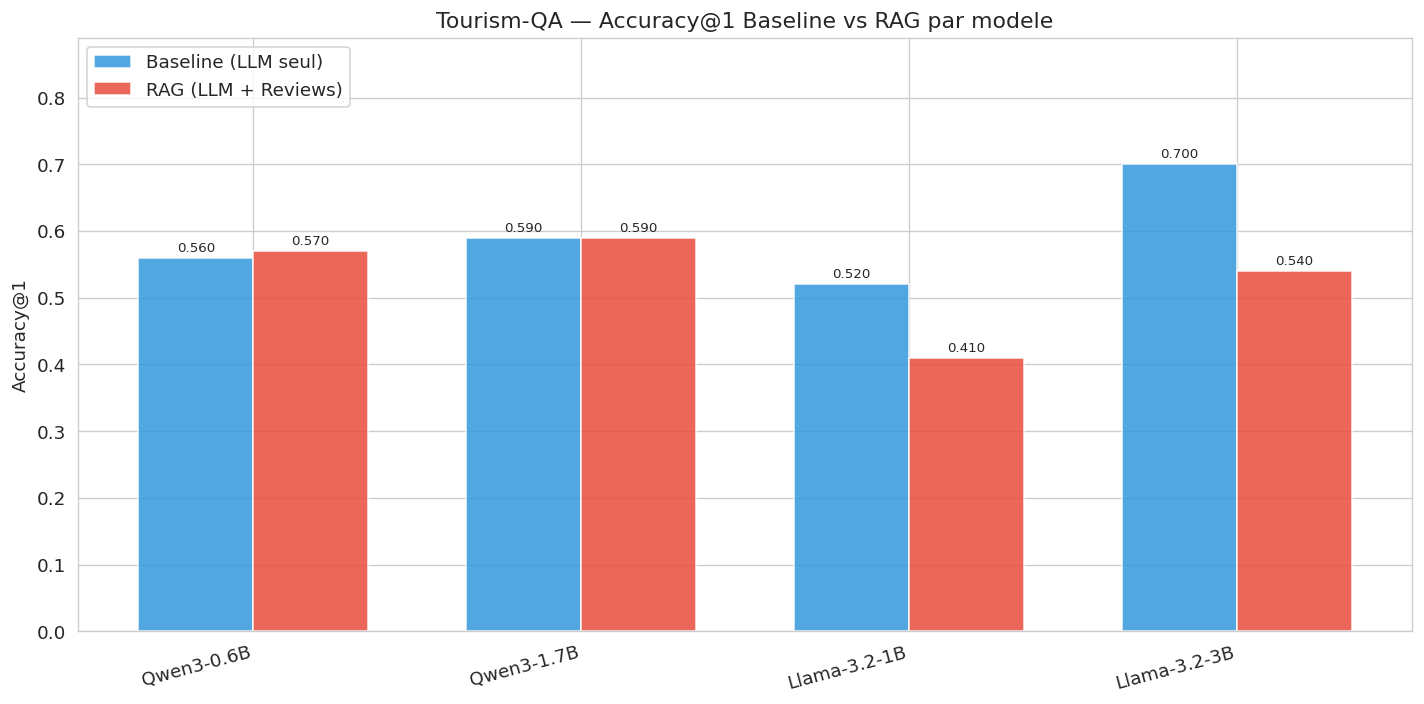
\includegraphics[width=\textwidth]{fig1_poi_accuracy_baseline_vs_rag.png}
    \end{column}
  \end{columns}

  \vspace{0.15cm}

  \begin{alertblock}{Paradoxe Tourism-QA}
    \begin{itemize}
      \item Hit Rate = \textbf{0.48} ($\times$8 vs GeoSQA/GKMC) -- le retriever fonctionne
      \item Pourtant, le RAG d\'egrade massivement les mod\`eles Llama (-21 \`a -23\,\%)
      \item Les mod\`eles Qwen r\'esistent au contexte non pertinent
    \end{itemize}
  \end{alertblock}
\end{frame}

\begin{frame}{Tourism-QA -- Exemples qualitatifs (Qwen3-0.6B)}
  \begin{table}
    \centering
    \small
    \begin{tabular}{@{} p{4cm} p{2.5cm} p{2.5cm} c @{}}
      \toprule
      \textbf{Question} & \textbf{Baseline} & \textbf{RAG} & \textbf{Effet} \\
      \midrule
      \rowcolor{green!8}
      Shopping femme Manhattan pas cher & Pasquale Jones & \textbf{Century 21} & \positif{Correction} \\
      \rowcolor{green!8}
      Restaurant Rome quartier Scalini & La Paila & \textbf{La Pancia Felice} & \positif{Correction} \\
      \rowcolor{green!8}
      Bar pour d\^iner 2\textsuperscript{e} Avenue NY & Vague & \textbf{Mermaid Inn} & \positif{Correction} \\
      \midrule
      \rowcolor{red!6}
      Italian food New York & Le Gavroche & Quay Bar & \negatif{Hallucination} \\
      \rowcolor{red!6}
      Mariage Londres 5 ans & \textbf{Le Gavroche} & Petrus & \negatif{D\'egradation} \\
      \bottomrule
    \end{tabular}
  \end{table}

  \vspace{0.2cm}

  \begin{itemize}
    \item \positif{Corrections}\,: le retriever r\'ecup\`ere les reviews du bon POI
    \item \negatif{D\'egradations}\,: reviews d'un autre POI $\to$ le mod\`ele est induit en erreur
  \end{itemize}
\end{frame}

\begin{frame}{Validation du mismatch linguistique}
  \begin{table}
    \centering
    \begin{tabular}{@{} l c c c @{}}
      \toprule
      \textbf{Dataset} & \textbf{HR@5 corpus FR} & \textbf{HR@5 corpus EN} & \textbf{Facteur} \\
      \midrule
      GeoSQA & 0.060 & 0.175 & $\times$2.9 \\
      GKMC & 0.075 & 0.190 & $\times$2.5 \\
      \bottomrule
    \end{tabular}
  \end{table}

  \vspace{0.4cm}

  \begin{block}{Conclusion}
    \begin{itemize}
      \item Le corpus EN multiplie le Hit Rate par \textbf{2.5 \`a 2.9}
      \item BGE-m3 encode correctement les questions -- c'est le \textbf{corpus FR} qui est inadapt\'e
      \item Mais sur GKMC, un meilleur retrieval ne suffit pas\,: les mod\`eles poss\`edent d\'ej\`a les connaissances en m\'emoire param\'etrique
    \end{itemize}
  \end{block}
\end{frame}

% ============================================================
% 6. ANALYSE FACTORIELLE
% ============================================================
\section{Analyse factorielle crois\'ee}

\begin{frame}{Facteur 1 -- Taille du mod\`ele}
  \begin{columns}[T]
    \begin{column}{0.52\textwidth}
      \begin{table}
        \centering
        \scriptsize
        \begin{tabular}{@{} l l c c c @{}}
          \toprule
          \textbf{Fam.} & \textbf{Dataset} & \textbf{Petit} & \textbf{Grand} & \textbf{$\Delta_{rel}$} \\
          \midrule
          \multirow{3}{*}{Qwen}
            & GeoSQA & 0.260 & 0.335 & \positif{+28.8\,\%} \\
            & GKMC & 0.415 & 0.605 & \positif{+45.8\,\%} \\
            & Tourism & 0.570 & 0.590 & \positif{+3.5\,\%} \\
          \midrule
          \multirow{3}{*}{Llama}
            & GeoSQA & 0.205 & 0.230 & \positif{+12.2\,\%} \\
            & GKMC & 0.335 & 0.485 & \positif{+44.8\,\%} \\
            & Tourism & 0.410 & 0.540 & \positif{+31.7\,\%} \\
          \bottomrule
        \end{tabular}
      \end{table}
    \end{column}
    \begin{column}{0.46\textwidth}
      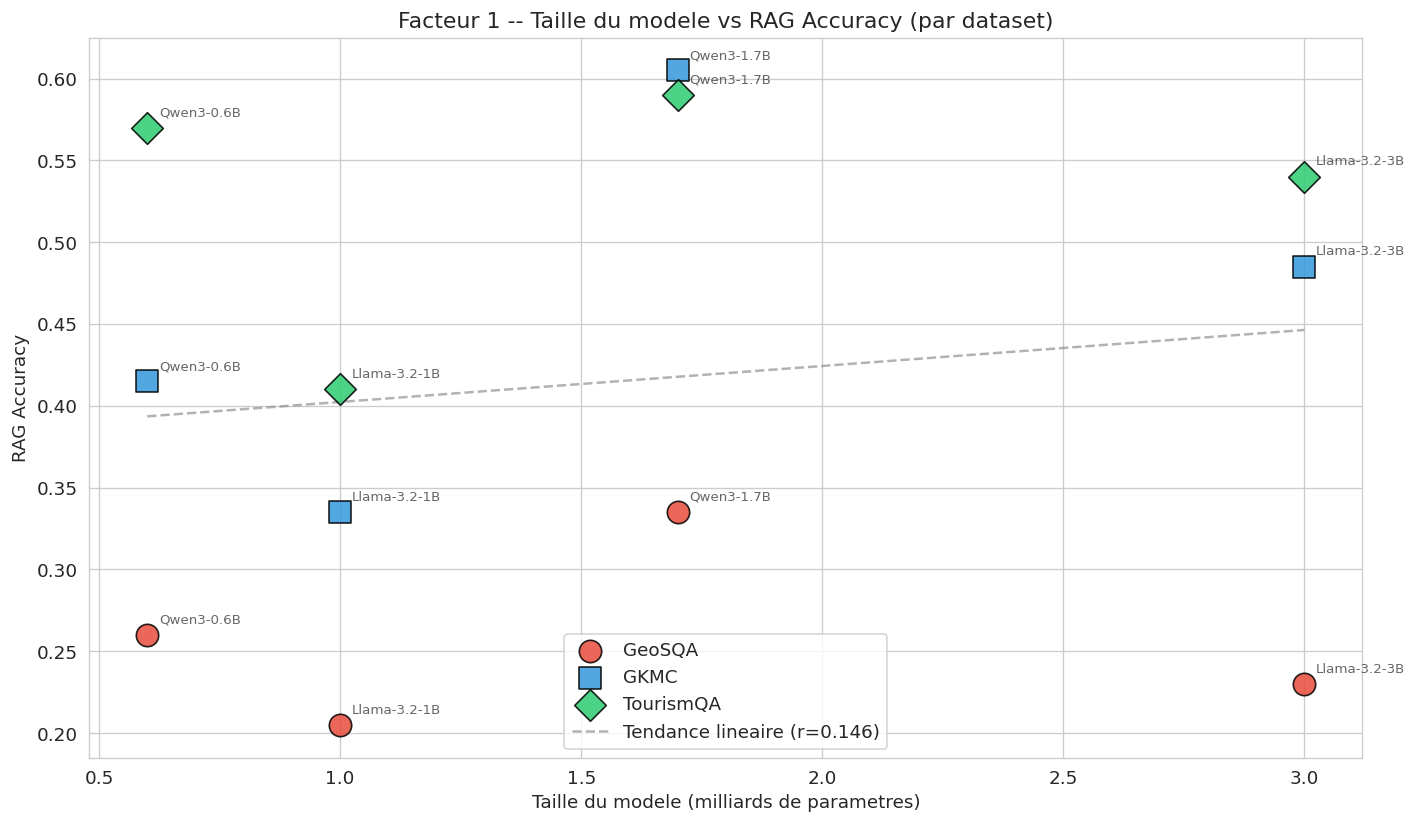
\includegraphics[width=\textwidth]{phase2d_fig1_taille_accuracy.png}
    \end{column}
  \end{columns}

  \vspace{0.3cm}

  \begin{block}{R\'esultat}
    La taille aide dans \textbf{6/6 configurations} sans exception, de +3.5\,\% \`a +45.8\,\%.
  \end{block}
\end{frame}

\begin{frame}{Facteur 2 -- Famille de mod\`ele}
  \begin{columns}[T]
    \begin{column}{0.50\textwidth}
      \begin{table}
        \centering
        \small
        \begin{tabular}{@{} l c c c @{}}
          \toprule
          & \textbf{GeoSQA} & \textbf{GKMC} & \textbf{Tourism} \\
          \midrule
          Qwen & 0.298 & 0.510 & 0.580 \\
          Llama & 0.218 & 0.410 & 0.475 \\
          \midrule
          $\Delta$ & \positif{+0.080} & \positif{+0.100} & \positif{+0.105} \\
          \bottomrule
        \end{tabular}
      \end{table}

      \vspace{0.2cm}

      Avantage Qwen\,: \textbf{+0.095} en moyenne, constant sur les 3 datasets.
    \end{column}
    \begin{column}{0.48\textwidth}
      
\includegraphics[width=\textwidth]{phase2d_fig2_famille_analyse.png}
    \end{column}
  \end{columns}
\end{frame}

\begin{frame}{Facteur 3 -- Impact du RAG}
  \begin{columns}[T]
    \begin{column}{0.55\textwidth}
      \begin{table}
        \centering
        \scriptsize
        \begin{tabular}{@{} l c c c c @{}}
          \toprule
          \textbf{Mod\`ele} & \textbf{GeoSQA} & \textbf{GKMC} & \textbf{Tourism} & \textbf{Moy.} \\
          \midrule
          Qwen3-1.7B & \negatif{-14.1} & \positif{+3.4} & 0.0 & \negatif{-3.6} \\
          Llama-3.2-3B & \negatif{-14.8} & \negatif{-14.2} & \negatif{-22.9} & \negatif{-17.3} \\
          Qwen3-0.6B & \negatif{-5.5} & \negatif{-1.2} & \positif{+1.8} & \negatif{-1.6} \\
          Llama-3.2-1B & \negatif{-25.5} & \positif{+1.5} & \negatif{-21.2} & \negatif{-15.0} \\
          \midrule
          \textbf{Moy.} & \negatif{-15.0} & \negatif{-2.6} & \negatif{-10.6} & \negatif{-9.4} \\
          \bottomrule
        \end{tabular}
      \end{table}
    \end{column}
    \begin{column}{0.43\textwidth}
      
\includegraphics[width=\textwidth]{phase2d_fig4_impact_rag_heatmap.png}
    \end{column}
  \end{columns}

  \vspace{0.3cm}

  \begin{alertblock}{Constat central}
    $\bar{\Delta}_{rel} = \mathbf{-9.4\,\%}$ -- Le RAG na\"if est \textbf{n\'egatif en moyenne}.\\
    3 cas positifs marginaux, 1 neutre, \textbf{8 d\'egrad\'es} sur 12 configurations.
  \end{alertblock}
\end{frame}

\begin{frame}{Classement global}
  \begin{columns}[T]
    \begin{column}{0.50\textwidth}
      \begin{table}
        \centering
        \small
        \begin{tabular}{@{} c l c c @{}}
          \toprule
          \textbf{\#} & \textbf{Mod\`ele} & \textbf{RAG Acc} & \textbf{Effic.} \\
          \midrule
          1 & Qwen3-1.7B & \textbf{0.510} & 0.300 \\
          2 & Llama-3.2-3B & 0.418 & 0.139 \\
          3 & Qwen3-0.6B & 0.415 & \textbf{0.692} \\
          4 & Llama-3.2-1B & 0.317 & 0.317 \\
          \bottomrule
        \end{tabular}
      \end{table}

      \vspace{0.2cm}

      \small
      Efficacit\'e = RAG Acc / Taille (B)\\
      Qwen3-0.6B\,: meilleur ratio qualit\'e/taille
    \end{column}
    \begin{column}{0.48\textwidth}
      
\includegraphics[width=\textwidth]{phase2d_fig7_radar.png}
    \end{column}
  \end{columns}
\end{frame}

% ============================================================
% 7. DISCUSSION
% ============================================================
\section{Discussion}

\begin{frame}{Pourquoi le RAG est-il inefficace\,?}
  \begin{enumerate}
    \item \textbf{Mismatch linguistique} (facteur dominant)
    \begin{itemize}
      \item Corpus FR, questions EN $\Rightarrow$ HR@5 = 0.060 -- 0.075
      \item Corpus EN valide l'hypoth\`ese (HR@5 $\times$2.5 \`a $\times$2.9)
    \end{itemize}

    \vspace{0.3cm}

    \item \textbf{Contexte non pertinent}
    \begin{itemize}
      \item Documents hors sujet inject\'es $\Rightarrow$ d\'etournement des connaissances internes
      \item Llama-Instruct particuli\`erement sensible (suit fid\`element le contexte fourni)
    \end{itemize}

    \vspace{0.3cm}

    \item \textbf{Exception partielle Tourism-QA}
    \begin{itemize}
      \item HR = 0.48 (corpus EN align\'e) mais RAG toujours n\'egatif en moyenne
      \item Qwen r\'esiste, Llama chute (-21 \`a -23\,\%) $\Rightarrow$ diff\'erence architecturale
    \end{itemize}
  \end{enumerate}
\end{frame}

\begin{frame}{Limites de l'\'etude}
  \begin{itemize}
    \item \textbf{4 mod\`eles $\leq$ 3B} uniquement -- les mod\`eles 7B+ n'ont pas pu \^etre charg\'es sur le GPU T4
    \item \textbf{Corpus monolingue FR} pour GeoSQA et GKMC -- inadapt\'e aux questions EN
    \item \textbf{RAG na\"if} uniquement -- pas de re-ranking, pas de r\'e\'ecriture de requ\^ete
    \item \textbf{200 questions} par dataset -- variance d'\'echantillonnage possible
    \item \textbf{Ministral incompatible} -- comparaison inter-familles limit\'ee \`a Qwen vs Llama
  \end{itemize}
\end{frame}

% ============================================================
% 8. CONCLUSION
% ============================================================
\section{Conclusion et perspectives}

\begin{frame}{Bilan synth\'etique}
  \begin{table}
    \centering
    \small
    \begin{tabular}{@{} l l @{}}
      \toprule
      \textbf{Constat} & \textbf{Valeur mesur\'ee} \\
      \midrule
      Meilleur mod\`ele global & Qwen3-1.7B (RAG Acc = 0.510) \\
      Meilleure efficacit\'e & Qwen3-0.6B (0.692 Acc/B) \\
      Impact RAG moyen & $\bar{\Delta}_{rel} = -9.4\,\%$ (n\'egatif) \\
      Taille aide (intra-famille) & 6/6 configurations \\
      Avantage Qwen vs Llama & +0.095 (constant) \\
      HR@5 corpus FR & 0.060 -- 0.075 \\
      HR@5 corpus EN (Tourism) & 0.48 \\
      \bottomrule
    \end{tabular}
  \end{table}
\end{frame}

\begin{frame}{Enseignements et perspectives}
  \begin{block}{4 enseignements cl\'es}
    \begin{enumerate}
      \item Le \textbf{RAG na\"if d\'egrade} les performances en moyenne ($\Delta_{rel}$ = -9.4\,\%)
      \item La \textbf{qualit\'e du retrieval} est le facteur d\'eterminant (HR@5 = 0.06 $\to$ 0.48)
      \item La \textbf{famille} importe davantage que la taille seule (Qwen $>$ Llama)
      \item \textbf{Qwen r\'esiste mieux} au contexte non pertinent que Llama
    \end{enumerate}
  \end{block}

  \vspace{0.15cm}

  \begin{block}{Perspectives}
    \begin{itemize}
      \item \textbf{Corpus multilingue} -- \'eliminer le mismatch linguistique
      \item \textbf{RAG avanc\'e} -- re-ranking par cross-encoder, r\'e\'ecriture de requ\^ete
      \item \textbf{Mod\`eles 7B+} en quantification 4-bit (QLoRA / bitsandbytes)
      \item \textbf{3\textsuperscript{e} famille} -- Mistral-7B-Instruct-v0.3 (architecture compatible)
    \end{itemize}
  \end{block}
\end{frame}

\begin{frame}[plain]
  \centering
  \vspace{2cm}
  {\Huge\color{upblue} Merci de votre attention}

  \vspace{1.5cm}

  {\large Questions\,?}

  \vspace{1.5cm}

  \small
  Code source\,: \url{https://github.com/Hiba-Lmoudden/GeoR2LLMs}\\
  Responsable\,: Lynda TAMINE-LECHANI (IRIT)
\end{frame}

\end{document}
